\documentclass[11pt, a4paper, DIV=12]{scrartcl}

% useful packages 
\usepackage{mathtools}
\usepackage{physics}
\usepackage{graphicx}					  
\graphicspath{{figs/}}

\usepackage{amssymb}
\usepackage{amsmath}
\usepackage{hyperref}
\usepackage[separate-uncertainty=true]{siunitx}
\usepackage{xcolor}
\usepackage{braket} % easy braket notation
\usepackage{enumitem}

\usepackage[backend=biber, sorting=none]{biblatex}
\bibliography{refs.bib}

% \numberwithin{equation}{section}

% New command and etc
\newcommand{\gag}{$\gamma$-$\gamma$ }

\title{Lab report\\K223 Nuclear \gag Angular Correlations}
\date{\today}
\author{Chenhuan Wang and Harilal Bhattarai}
\begin{document}
\maketitle

\begin{abstract}
	This is abstract.
\end{abstract}

\section{Introduction}

\section{Theory}
The partial decay width of $Z^0$ decay into fermion $f$ is
\begin{equation}
	\Gamma_f = \frac{ \sqrt{2} N_c^f}{12\pi} G_F M_Z^3 \left( (g_V^f)^2 + (g_A^f)^2  \right)
	\label{math:Gammaf}
\end{equation}
with
\begin{align*}
	g_V^f &= I_3^f - 2 Q_f \sin^2 \theta_W \\
	g_A^f &= I_3^f 
\end{align*}
One needs to be aware that $\Gamma_f$ contains contribution from both chiralities, and $I_3$ here refers to only the weak isospin of left-handed fermions (by definition right handed fermions have no weak isospin).

Partial cross section of $Z^0 \rightarrow f\bar{f}$ is given by~\cite{manual}
\begin{equation}
	\sigma_f(s) = \frac{12 \pi}{M_Z^2} \frac{s \Gamma_e \Gamma_f}{ (s-M_Z^2)^2 + (s^2 \Gamma^2_Z / M_Z^2)}
\end{equation}

In $ee \rightarrow ee$ scattering, two relevant channels have different angular dependences. For $s$-channel,
\begin{equation}
	\dv{\sigma}{\Omega}_s \sim (1 + \cos^2 \Theta)
	\label{math:diffCrossS}
\end{equation}
For $t$-channel,
\begin{equation}
	\dv{\sigma}{\Omega}_t \sim (1-\cos^2 \Theta)^{-2}
	\label{math:diffCrossT}
\end{equation}

\clearpage
\section{Setup}\label{sec:setup}

\subsection{Individual components}
\paragraph{Drift chamber}
is a type of gaseous ionization detector. As its name suggest, it detects ionizing particles by a electric field inside. When the gas atoms get ionized, the electron will transport to the anode and generate a signal. Especially near the anode wire, the electric field is so huge that the electron becomes ionizing itself and cause further discharge. This effect is called avalanche~\cite{leo}. Obviously, number of ions collected at anode depends strongly on the voltage put between anode and cathode.

\begin{figure}[htpb]
	\centering
	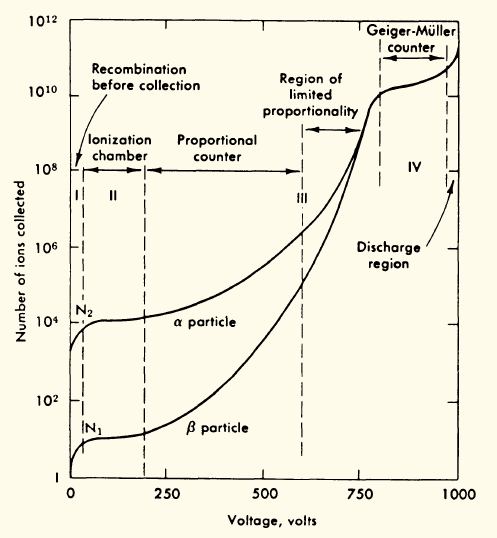
\includegraphics[width=0.5\linewidth]{voltage-diagram.png}
	\caption{Example diagram of number of ions versus applied voltage in a single wire gas chamber (taken from~\cite{leo}). Note that vertical axis is in logarithmic scale. }%
	\label{fig:voltage-diagram}
\end{figure}
An exemplar development of number of ions with increasing voltage is shown in figure~\ref{fig:voltage-diagram}. In this setup, we essentially want to saturate the gas chamber (thus to region IV in figure~\ref{fig:voltage-diagram}) so that it can reliably count the ionizing particles regardless of their energy.

In this experiment, there are three drift chamber modules, see figure~\ref{fig:setup-real}. In each of these, there are three layers of $88$ straws~\cite{manual}.

\paragraph{Scintillator and PMT}
work as external trigger here. They together are able to convert ionizing particle into relatively low energy photons (scintillator), convert photon into electrons using photoelectric effect, and finally with electric field to multiply the number of electrons to generate visible signals~\cite{wermes}. Here two such detectors are used, one on top of the drift chamber and on below~\cite{manual}, see figure~\ref{fig:setup-real}.

\paragraph{Shaper}
A shaper is a module which turns inputs pulse into logic signals of standard levels and fixed width~\cite{leo}.

\paragraph{TDC}
stands for Time-to-Digital Converter measures the time between two signals and gives the time difference of these two~\cite{leo}.

\paragraph{Coincidence unit}
determines if two or more logic signals overlap with each other within a preset time intervals and output signal if true and no signal if false. The present time is called resolving time. It can be implemented with a transmission gate or simply summing and passing through a discriminator~\cite{leo}.

\subsection{Whole setup}
\begin{figure}[ht]
	\centering
	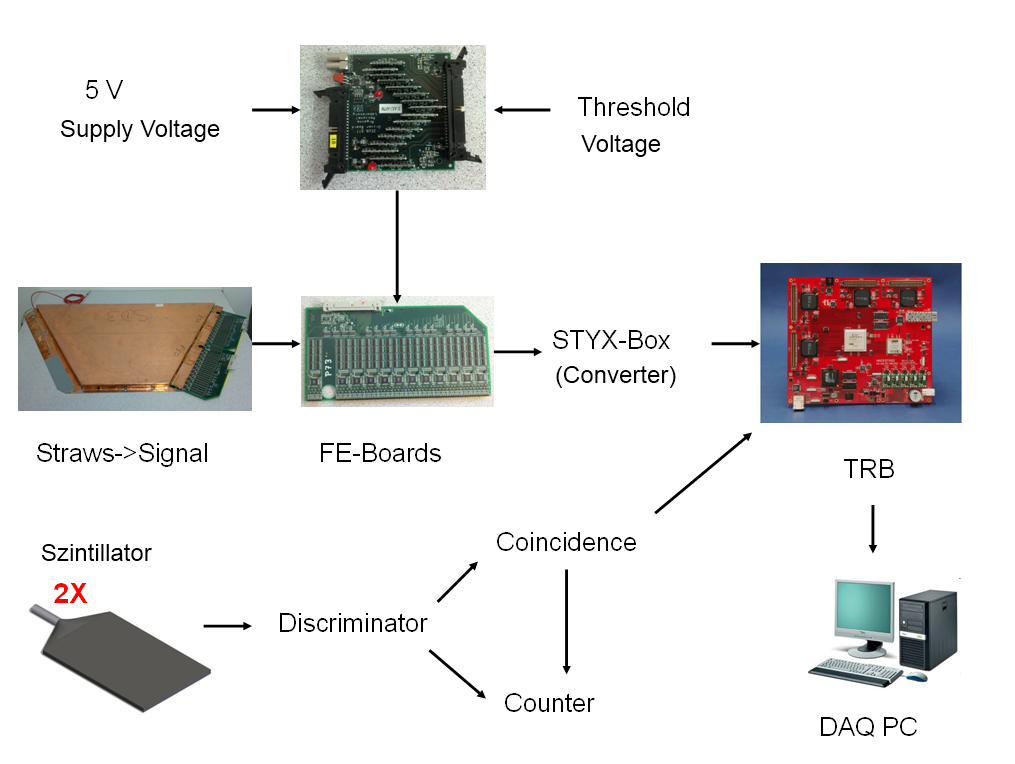
\includegraphics[width=0.6\linewidth]{setup-schematic.png}
	\caption{Schematics of the experiment setup~\cite{manual}.}%
	\label{fig:setup}
\end{figure}
Schematically the setup is like in figure~\ref{fig:setup}. The front end boards (FE-boards) are attached to the straws. The boards contain amplifiers, shapers and discriminators, so that as long as input signal pass a set threshold, a logic signal is generated. The threshold voltage can be set on an external power supply. As for the trigger part, the signal will need to pass discriminators (to filter out noises) and goes to a coincidence unit. The coincidence unit makes sure that an event is only recorded when it flies through both scintillators. In the end, signals from straw modules and scintillator units go into TRB board and to the PC~\cite{manual}.

The actual setup is shown in figure~\ref{fig:setup-real}. Straw modules with FE-boards are the copper layer between the two plastic bags, which are the triggers. Several other electronics are on the rack on the right side of figure~\ref{fig:setup-real}.

\begin{figure}[ht]
	\centering
	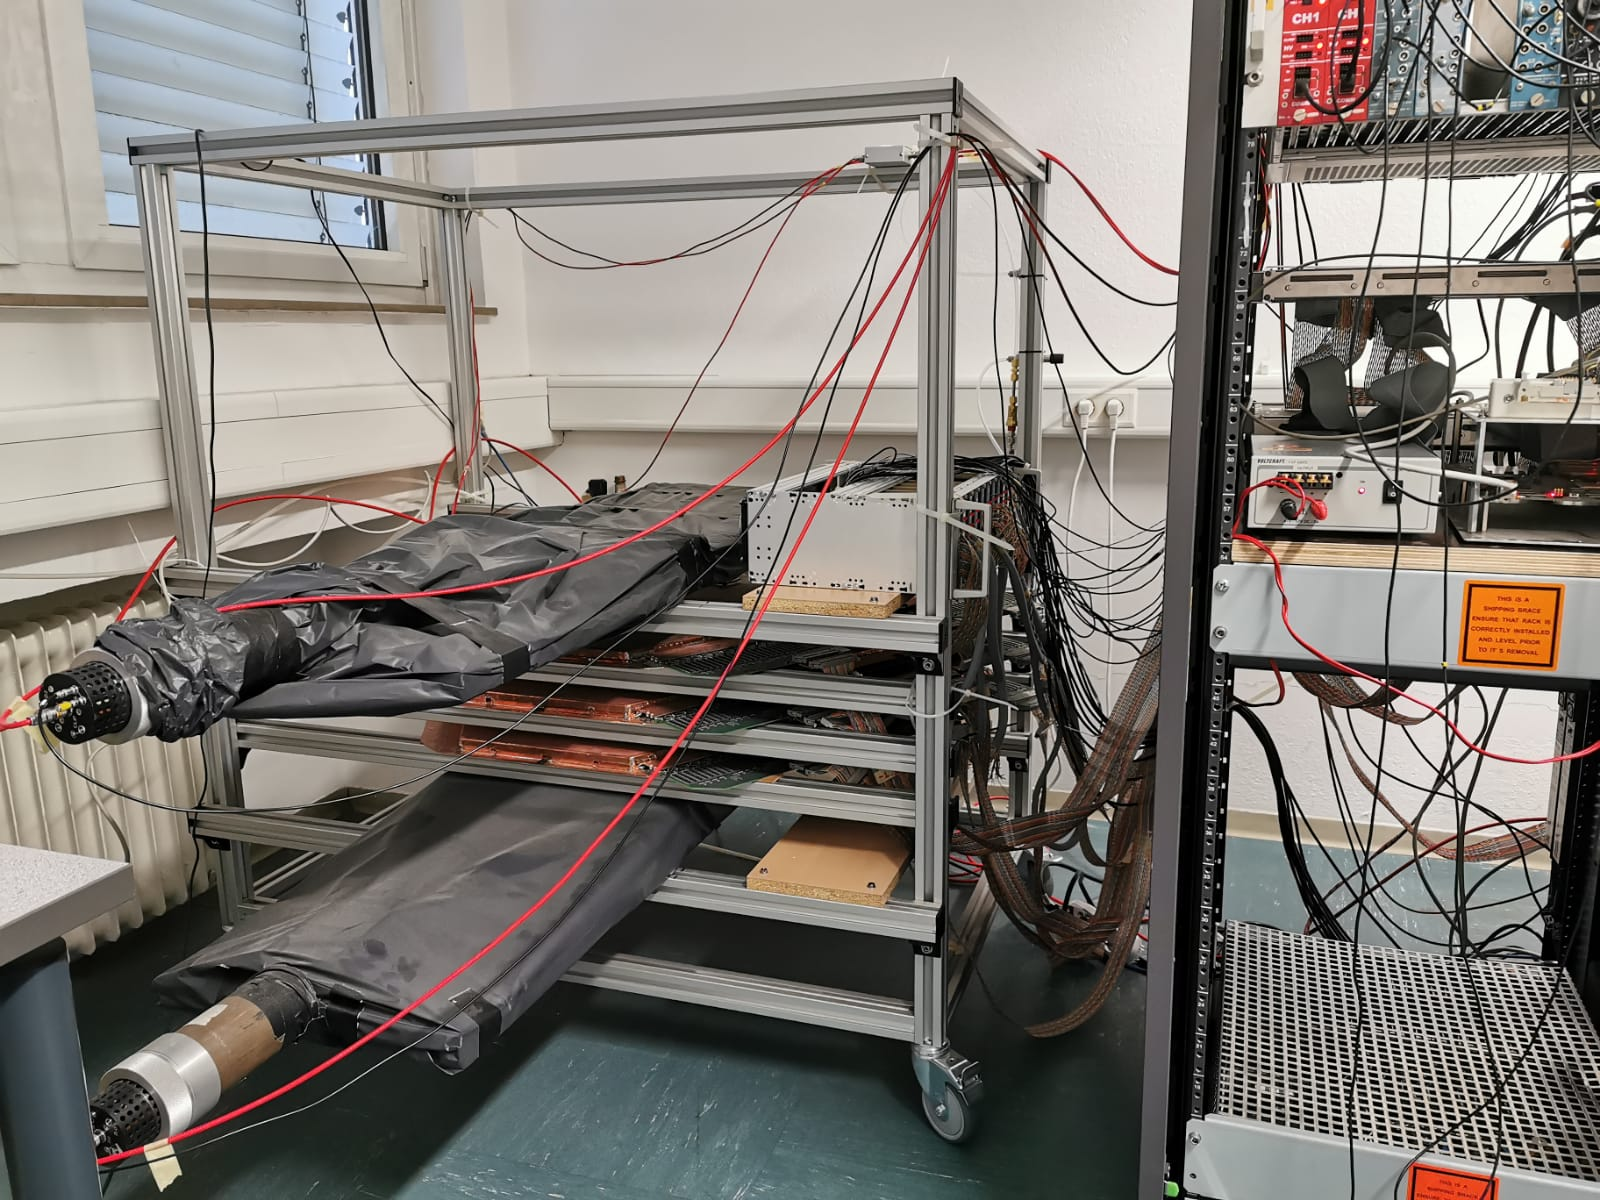
\includegraphics[width=0.6\linewidth]{setup-reallife.jpeg}
	\caption{The actual setup}%
	\label{fig:setup-real}
\end{figure}

\clearpage
\section{Lensing analysis} 
\paragraph{Calculation with accepted value of $H_0$}
Since the redshifts of lens and source system are known, one can from image separation determine the velocity dispersion in SIS model. Angular distances should be computed also by equation.~\ref{math:Dangular2}. Here the cosmological parameters are taken from~\cite{planck}
\begin{equation*}
	\Omega_m = \num{0.3089 +- 0.0062}, \quad \Omega_\Lambda=\num{0.6911 +- 0.0062}
\end{equation*}
For simplicity, errors in these parameters are not propagated in further analysis (almost negligible). For this part, currently accepted value of $H_0$ is used.

Image separation can be used to compute Einstein radius. Results of \verb|galfit| are in pixels, so they need to be converted to angles first. As given in~\cite{alfa-manual}, the field of view of Cassegrain focus is $21'\times14'$, meaning one pixel corresponds to $0.4''$. Image separation can be expressed by Einstein radius with equation.~\ref{math:imSep}. The separation in pixels and in radians are then
\begin{align*}
	\Delta r &= \num{6.60 +- 0.079} \, \text{(pixels)} \\
	\Delta \theta &= (\num{1.281 +-0.015}) \cdot 10^{-5} = 2 \theta_E
\end{align*}
Here the error is properly propagated using
\begin{align*}
	\sigma_{\Delta r} ^2 &= \left( \pdv{\Delta r}{x_A}  \right)^2 \sigma_{x_A}^2 + \left( \pdv{\Delta r}{y_A}  \right)^2 \sigma_{y_A}^2 + \left( \pdv{\Delta r}{x_B}  \right)^2 \sigma_{x_B}^2 + \left( \pdv{\Delta r}{y_B}  \right)^2 \sigma_{y_B}^2 \\
								&= \frac{1}{(\Delta r)^2} \left[ (x_A - x_B)^2(\sigma_{x_A}^2 + \sigma_{x_B}^2) + (y_A - y_B)^2 (\sigma_{y_A}^2 + \sigma_{y_B}^2) \right]
\end{align*}

With equation.~\ref{Equ:ThetaE}, one finds
\begin{equation}
	\sigma_v = (\num{9.913 +- 0.597 })\cdot 10^{-4} c
\end{equation}
where the error is given by
\begin{equation*}
	\sigma_{\sigma_v} = \frac{\sigma_v}{2\theta_E} \sigma_{\theta_E}
\end{equation*}

According to equation.~\ref{math:projMass}, projected mass inside Einstein radius is computed to be
\begin{equation}
	M(\theta < \theta_E) = (\num{5.766 +- 0.139}) \cdot 10^{11} M_\odot
\end{equation}
This has similar magnitude as the estimated mass of milky way ($\sim \num{1e12} M_\odot$)~\cite{Grand_2019}. The error is propagated to be
\begin{equation*}
	\sigma_{M} = \frac{2M}{\theta_E} \sigma_{\theta_E}
\end{equation*}

\paragraph{Determination of $H_0$}

\section{Conclusion}\label{sec:conclusion}
In this experiment, we measured angular correlation between two photons emitted from ${}^{60}\text{Co}$. Then, the data gets fitted with the theoretical prediction function and  the angular correlation coefficients are calculated:  $ A_{22}= \num{0.0849 +- 0.0057} $ and $A_{44}=\num{-0.0002 +- 0.0063} $. The non-zero values of these two angular correlation coefficients provide strong evidence for an angular correlation between two gamma rays emitted in 420 cascade of $ ^{60}\text{Co} $. Via curve fitting, we can conclude that other types of cascade (020,121, 220, and 320) are basically $100\%$ excluded.

Further investigation reveals that measured values differ from prediction by $4\sigma$ due to unknown systematic errors in the setup. One of these systematic errors could very well be in electronics. Geometry of the setup could be measured and investigated more. As mentioned before, the resolving time can be lowered a bit. But it should not have huge impact on determination of angular correlation coefficients. 

\section{Acknowledgement}
We would heartly acknowledge the Bonn-Cologne Graduate School of Physics and Astronomy (BCGS) for the opportunity to perform the experiment. We would like to express our gratitude and appreciation for Dr. Christian Honisch for the tutoring, encouragement, and guidance throughout the experiment.


\clearpage
\printbibliography
\end{document}
